\documentclass{beamer}
\usepackage{tikz}
\usepackage{caption}
\usepackage[
    backend=biber,
    bibstyle=numeric,
    citestyle=authoryear,
    sorting=ynt,
    natbib
]{biblatex}
\addbibresource{references.bib} % This command is used instead of \bibliography{references.bib}

\usetikzlibrary{positioning}
\usetikzlibrary{calc}
\usetikzlibrary{shapes, positioning, arrows.meta, fit}
\captionsetup{justification=centering}

\usetheme{Copenhagen}
\usecolortheme{default}
\setbeamertemplate{navigation symbols}{}

\DeclareMathOperator*{\argmax}{arg\,max} 
\DeclareMathOperator*{\argmin}{arg\,min}
\newcommand{\indep}{\perp \!\!\! \perp}
\newcommand\norm[1]{\lVert#1\rVert}
\newcommand{\q}{q}
\newcommand{\ml}{k}
\newcommand{\btheta}{\theta}
\newcommand{\la}{\psi}
\newcommand{\Sn}{S^n}
\newcommand{\lib}{\Psi}
\newcommand{\lone}{\mathcal{L}}
\newcommand{\empmod}{\mathcal{P}_{\text{emp}}}
\newcommand{\meta}{\phi}
\newcommand{\Meta}{\Phi}
\newcommand{\esl}{\Sigma}
\DeclareMathOperator{\expit}{expit}




% \title[About Beamer] %optional
\title{Super Learners}
\subtitle{and their oracle properties}
\author[Jinyang Liu (sqf320)]{Jinyang Liu (sqf320)}

\institute[UCPH] % (optional)
{
  Department of Mathematical Sciences\\
  University of Copenhagen
}

\date[VLC 2023]{June 2023}


%End of title page configuration block
%------------------------------------------------------------
%The next block of commands puts the table of contents at the 
%beginning of each section and highlights the current section:

\AtBeginSection[]
{
  \begin{frame}
    \frametitle{Table of Contents}
    \tableofcontents[currentsection]
  \end{frame}
}

%------------------------------------------------------------
\begin{document}


\frame{\titlepage}
%---------------------------------------------------------
\begin{frame}
    \frametitle{Introduction}
    \begin{block}{Binary regression}
        Let $ O = (Y, X) $ be an observation for $ Y \in \{0,1\} $ and $ X \in \mathcal{X}$ for $ \mathcal{X} \subseteq \mathbb{R}^{d} $. We assume that $ O \sim P $ for some $ P \in \mathcal{P} $.
    \end{block}
    Let $ \Theta = \{\btheta \mid \btheta : \mathcal{X} \to [0,1] \text{ measurable}\} $ be the set of \textbf{regression functions}. We would like to \textbf{estimate} a function $ \btheta \in \Theta $ such that the mean squared error (MSE) or risk
        $$
            R(\btheta , P) = \int L(O, \btheta) dP = \int (Y - \theta(X))^2 d P  
        $$
        is minimized. It turns out that the conditional expectation $$ x \mapsto E(Y \mid X = x) = P(Y \mid X = x) $$ is what minimizes the MSE. We refer to it as the \textbf{regression}.  
\end{frame}

\begin{frame}
    \frametitle{Example of a regression function}
    \begin{figure}[H]
        \centering
        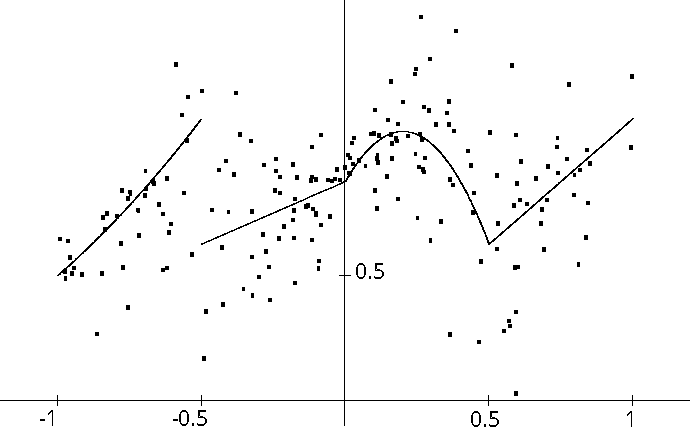
\includegraphics[width=0.85\textwidth]{figures/trueregression}
        \caption{Example of a pathological regression that can be difficult to learn using parametric techniques. Here a continuous outcome $ Y $ is plotted against a single continuous covariate $ X $ \citep{gyorfi2002distribution}.}
    \end{figure}
\end{frame}

\begin{frame}
    \frametitle{Linear approximation}
    \begin{figure}[H]
        \centering
        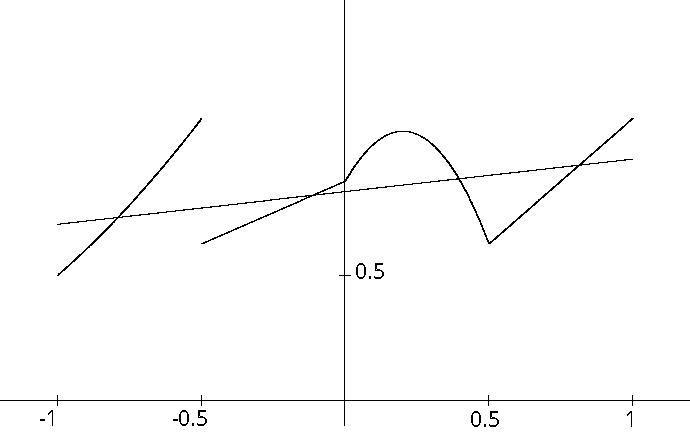
\includegraphics[width=0.85\textwidth]{figures/linearestimate}
        \caption{Approximating the regression using linear regression, which is very biased \citep{gyorfi2002distribution}.}
    \end{figure}
\end{frame}

\begin{frame}
    \frametitle{Terminology}
    We observe $ D_n = (O_1 , \dots , O_n) $, upon which we apply our \textbf{learning algorithms}  
    \begin{definition}[Learning algorithm]
        A learning algorithm is a measurable map $ \la : \mathcal{O}^{n} \to \Theta $ for $ n \in \mathbb{N} $. 
    \end{definition}
    We assume that the $ \la $ is well-defined for all $ n \in \mathbb{N} $ and that the ordering of the observations does not matter.  
    \begin{definition}[Learner or fitted learner]
        Let $ \la $ be a learning algorithm, a learner is the outcome of applying $ \la $ to our data $ D_n $ denoted as $ \la(D_n) $, which is a map in $ \Theta $.
    \end{definition}
    We usually have a \textbf{library of learning algorithms}, 
    \begin{align*}
        \lib = \{\la_{\q} \mid 1 \leq \q \leq\ml \},
    \end{align*}
    for which we can use to estimate the regression.  
\end{frame}

\begin{frame}
\frametitle{$ K $-fold Cross-validation}
There is a one-to-one correspondance between our data $ D_n $ and the empirical measures over $ n $ observations
\begin{align*}
    P_n = \sum_{i = 1}^{n} \delta_{O_i},
\end{align*}
where $ \delta_{O_i} $ is the Dirac measure over $ O_i $. $ K $-fold cross-validation splits $ D_n $ into \textbf{validation} and \textbf{training} sets. Index the validation sets by $ s \in \{1, \dots , K\} $ and denote the empirical measure over the validation set $ s $ as 
\begin{align*}
    P_{n,s}^{1} := \frac{1}{n_1} \sum_{i: s(i) = s} \delta_{O_i}, \qquad P_{n,s}^{0} := \frac{1}{n_0} \sum_{i: s(i) \neq s} \delta_{O_i}. 
\end{align*}
Here $ s(i) $ denotes whether $ O_i$ is in the validation set $ s $, and $ n_1, n_0 $ are the number of observations in the validation and training sets respectively. 
\end{frame}

\begin{frame}
\begin{exampleblock}{$ K $-fold Cross-validation Procedure}
Cross-validation is used to evaluate each algorithm, and is the central idea of the \textbf{super learner}:
    \begin{enumerate}
        \item Randomly split $ D_n $ into $ K $ disjoint and exhaustive validation sets
        \item For each $ s \in \{1, \dots , K\} $ fit each $ \la \in \lib $ on the training data $ P_{n, s}^{0} $ and obtain $ \la(P_{n, s}^{0}) $ 
        \item Use $ \la(P_{n, s}^{0}) $ to predict on the validation set to obtain \textbf{level-1 covariates} $ Z_i = \left(\la_1(P_{n, s(i)}^{0})(X_i), \dots ,\la_\ml(P_{n, s(i)}^{0})(X_i)\right)  $
        \item Calculate the MSE of $ \la $ on the validation set for $ s \in \{1, \dots, K \}$ 
            $$ R(\la(P_{n, s}^{0}) , P_{n, s}^{1}) = \frac{1}{n_1} \sum_{i : s(i) = s} \left(Y_i - \la(P_{n, s}^{0})(X_i)\right)^2 $$ 
    \end{enumerate}
\end{exampleblock}
\end{frame}

\begin{frame}
\frametitle{Discrete Super Learner}
Cross-validation allows us to select the algorithm with the lowest \textbf{empirical risk
}
\begin{align*}
    \hat{\la}_n := \argmin_{\la \in \lib} \frac{1}{K} \sum_{s = 1}^{K} R(\la(P_{n, s}^{0}) , P_{n, s}^{1}),  
\end{align*}
also known as the \textbf{cross-validation selected algorihm}. The \textbf{discrete super learner} is simply the cross-validation selected algorithm fitted on the entire dataset 
\begin{align*}
    X \mapsto \hat{\la}_n(P_n)(X).
\end{align*}
It is compared to the \textbf{oracle selected learning algorithm} that has the true minimum risk
\begin{align*}
    \tilde{\la}_n := \argmin_{\la \in \lib} \frac{1}{K} \sum_{s = 1}^{K} R(\la(P_{n, s}^{0}) , P).  
\end{align*}

\end{frame}

\begin{frame}
    \frametitle{Discrete Super Learner: Oracle Equivalence}
\begin{corollary}[Asymptotic equivalence] \label{cor:dslasymptoticequivalence}
    If there exists an $ \varepsilon > 0 $ such that 
   \begin{align*}
       E_{D_n} \frac{1}{K} \sum_{s = 1}^{K} R(\tilde{\la}_n(P_{n, s}^{0}), P) > \varepsilon \qquad \text{for all } n \in \mathbb{N},
   \end{align*}
   and if $ n_1 = f(n) $ for some polynomial function $ f $, then the risk of the super learner is asymptotically equivalent with the risk of the oracle selected learner, that is
   \begin{align*}
       \lim_{n \to \infty} \frac{E_{D_n} E_{\Sn} R(\hat{\la}_n(P_{n, \Sn}^{0}), P)}{E_{D_n} E_{\Sn} R(\tilde{\la}_n(P_{n, \Sn}^{0}), P)} = 1.
   \end{align*}
\end{corollary}
\end{frame}


\end{document}
